%!TEX root = ../thesis.tex
\section{Rehabilitace hlasu po totální laryngektomii}
\label{chap:cause:treatment}

Nesporná výhoda totální laryngektomie neoddiskutovatelně spočívá v~odstranění
primárního nádorového onemocnění. Následky operace však způsobí obrovský
zásah do kvality života pacienta. Okem nejviditelnější změnu představuje
přítomnost otvoru na krku po provedeném operačním zákroku a s~ním spojený způsob dýchání.
Do uměle vyvedené průdušnice je přímo vdechován vzduch z okolního prostředí a nedochází tak  k~jeho přirozeně probíhající filtraci, ohřevu ani přirozenému zvlhčování. Toto má za následek vyšší náchylnost pacientů  k~respiračním onemocněním.

Lze se domnívat, že pro samotného pacienta je jedním z nejobtížnějších úkolů vypořádat se s~trvalou
ztrátou vlastního hlasu. Z toho důvodu se již samotný autor operačního zákroku doktor
Billroth zaobíral otázkou rehabilitace hlasu. Jeho první pokusy s~kovovou
tracheostomickou kanylou sice umožňovaly pacientovi hovořit, ale svou
konstrukcí pacienta spíše ohrožovaly na životě, proto se častěji využívala
metoda tzv. jícnového hlasu \cite{Sebova-Sedenkova2006}. Ve stejnou
dobu, tedy začátkem minulého století, se začaly objevovat také %první interní a externí
hlasové aparáty. V~současnosti se rehabilitace hlasu provádí s~využitím: %následujících metod:

\begin{itemize}
  \item \textbf{foniatrických metod}, mezi které patří metoda jícnového hlasu a využití elektrolarynxu,
  \item \textbf{chirurgicko-protetickým způsobem}, který spočívá v~opětovném propojení průdušnice a jícnu,
  \item \textbf{vytvoření hrtanu podobných struktur chirurgickým způsobem},
  \item \textbf{transplantace hrtanu}.
\end{itemize}

\noindent Může se zdát, že je  k~dispozici relativně široká škála
možností, jak pacientovi vrátit schopnost vyjadřování pomocí mluvené řeči.
Ovšem je nutné si uvědomit, že výběr konkrétní metody závisí na stavu
a možnostech pacienta. Jinými slovy, ne každá metoda je vhodná pro každého pacienta
a žádná z~metod není univerzální.

\subsection{Foniatrické metody} % (fold)
\label{chap:cause:treatment:foniatric}

Nevyhnutelným důsledkem odstranění hrtanu je ztráta hlasu. Neznamená to ale, že by byla
úplně eliminována schopnost produkovat řeč. V~procesu vytváření hlasu zastává
odstraněný orgán pouze (i když velmi zásadní) roli generátoru zvuku. Zbylé
orgány, jako například hrdelní, nosní a ústní dutina, zůstávají nedotčeny a mohou i
nadále plnit svou funkci. Logicky se tak nabízí myšlenka nahradit chybějící
zdroj zvuku jiným. Tento princip využívají metoda jícnového hlasu a produkce řeči s~využitím
elektrolarynxu.

\subsubsection{Jícnový hlas} % (fold)
\label{chap:cause:treatment:foniatric:esophageal}

První zmínky o využívání jícnového hlasu se datují do roku 1922, kdy prof. MUDr. Miloslav Seeman
\cite{seeman1922speech} potvrdil domněnku, že funkci štěrbiny mezi hlasivkami (rima
glottidis) přebírá tzv. pseudoglottis, která se vytváří na úrovni horního
jícnového svěrače, a vypracoval metodiku vytváření jícnového
hlasu.

Princip tvorby jícnového hlasu spočívá v~tom, že se vzduch neplní do plic, ale do jícnu.
Takto si pacient připravuje potřebný vzduch  k~následné
eruktaci\footnote{eruktace - latinsky název pro proces říhání (popřípadě
krkání), při kterém dochází  k~úniku plynů pocházejících ze žaludku dutinou
ústní.} vzduchu a produkci řeči. Vlastní jícnový hlas vzniká na přechodu
jícnu a hypofaryngu (spodní část hltanu). Následně v~oblasti horního jícnového
zúžení dochází  k~rozkmitání sliznice a podslizniční vrstvy, a tedy  k~produkci zvuku,
který je následně modulován stejně jako v~případě přirozené produkce řeči.
Princip tvorby \uv{základního} tónu jícnového hlasu je znázorněn na obr.
\ref{fig:cause:treatment:esophageal}.

\begin{figure}[htb]
  \begin{center}
    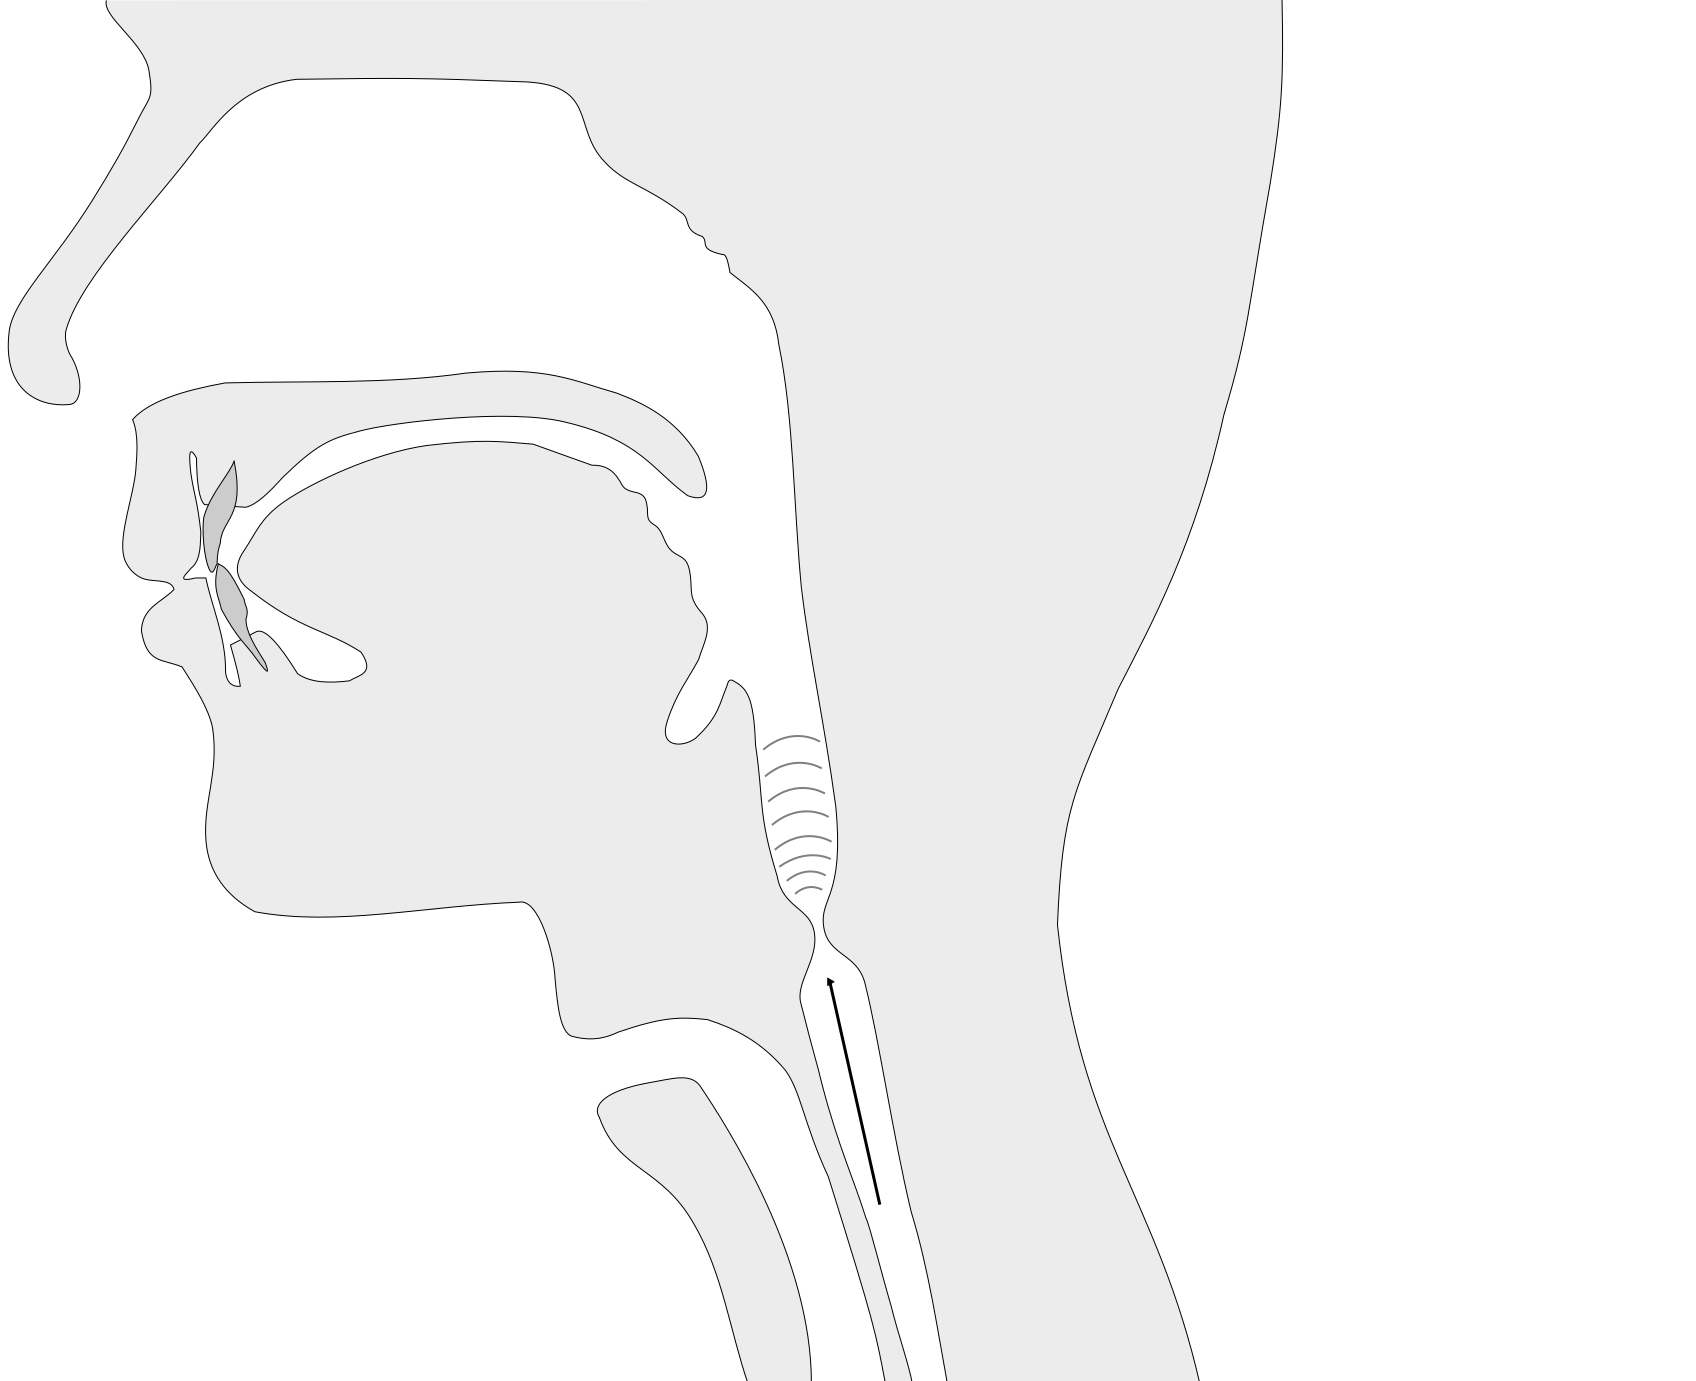
\includegraphics[width=0.6\linewidth]{ch3-cause/figures/esophageal}
    \caption[Princip produkce jícnového hlasu.]{Princip produkce jícnového hlasu. Průchodem vzduchu přes zúžení vzniká základní tón jícnového hlasu.}
    \label{fig:cause:treatment:esophageal}
  \end{center}
\end{figure}

Na základě toho, jakým způsobem je jícen plněn vzduchem, rozlišujeme metodu \textbf{aspirační} a metodu \textbf{injekční}. Zatímco aspirační metoda spočívá v~plnění jícnu vzduchem pomocí polykání, u injekční metody je za tímto účelem využíván kořen jazyka, pomocí něhož je vzduch vtlačován do jícnu. Následný princip produkce hlasu je pro oba případy shodný. Injekční princip plnění jícnu vzduchem je využíván pacienty, kterým byla
při laryngektomii odstraněna jazylka. V~těchto případech nelze jícen naplnit aspirační cestou.

Proces učení jícnového hlasu by měl začít co možná nejdříve po operaci. Pokud
je to možné, tak se s~výukou začíná ještě za pobytu pacienta na ORL klinice
nebo krátce po propuštění. V~první fázi se pacient učí pouze slabiky
sestávající z explosivy a souhlásky. Postupně se však přidávají slabičné
shluky, které sice nedávají smysl, ale pomáhají v~osvojení potřebné techniky.
V případě úspěšného zvládnutí se přistupuje  k~nácviku frází a souvislé řeči.
Potřebnou dobu  k~nácviku jícnového hlasu nelze přesně určit, protože je
závislá na mnoha faktorech. V~literatuře se uvádí, že pro úspěšné osvojení techniky jícnového hlasu je potřeba 30 až 50 hodin velmi intenzivního tréninku \cite{Brown2003}. Míra úspěšnosti nácviku srozumitelného hlasu se uvádí v~rozsahu 14\%-75\%. %Takto obrovský rozsah značí o mnoha faktorech, které mohou ovlivnit úspěšné osvojení jícnového hlasu.
Mezi možné příčiny, které mohou významně ovlivnit zvládnutí techniky jícnového hlasu, patří
fyziologické potíže, anatomické problémy, psychologické problémy, nebo jednoduše
neadekvátní podpora při řečové terapii \cite{Brown2003}. Významnou roli také
hraje snaha a odhodlání samotného pacienta.

Nepopiratelnou výhodou využití metody jícnového hlasu je, že při rehabilitaci hlasu není pacient závislý na lékaři. Navíc po chirurgickém zásahu je zajištěno permanentní oddělení dýchacích a
polykacích cest, je tedy eliminováno riziko vniknutí potravy do dýchacích cest.
Další nespornou výhodou pro pacienty, kteří ovládají techniku jícnového hlasu, je bezesporu to, že mají při mluvení
volné obě ruce. Za nevýhodu lze obecně považovat nižší srozumitelnost produkovaného hlasu.
Ta je způsobena tzv. \uv{břišním} zabarvením, ke kterému zcela jistě při produkci řeči prostřednictvím metody jícnového hlasu  dochází, a dále nízkou intenzitou hlasu a krátkou výdrží mluvčího při tvorbě tónu. Za negativum se dá také považovat množství pacientem vynaloženého úsilí potřebného  k~osvojení
techniky. Velmi často se také mluvčí ostýchají jícnový hlas používat, protože
mají pocit, že je společensky nevhodné dorozumívat se formou blízkou říhání. Z
tohoto důvodu se odhaduje, že v~běžném životě využívá jícnový hlas pouze 20\% -30\%
pacientů, kteří se začali tuto techniku učit \cite{Hradecka2007}.

% subsubsection jícnový_hlas (end)

\subsubsection{Využití elektrolarynxu} % (fold)
\label{chap:cause:treatment:foniatric:elektrolarynx}

Rehabilitace hlasu za pomoci přídavného zařízení, nazývaného elektrolarynx, se řadí mezi tzv. elektromechanické
metody. Princip metody spočívá v~přikládání speciálního zařízení obsahujícího generátor zvuku do oblasti spodiny úst. Generátor zvuku, který je součástí elektrolarynxu, napomáhá přenosu zvuku a vibrací nejen do dutiny ústní, ale i do přilehlých artikulačních orgánů. Následně je pacient schopen běžným způsobem artikulovat, a tedy i hovořit. Princip vytváření hlasu pomocí elektrolarynxu je ukázán na obr. \ref{fig:cause:treatment:electrolarynx}.



%Princip spočívá v~přikládání zařízení, které obsahuje generátor zvuku
%nazývaný elektrolarynx. Přiložením do oblasti spodiny úst a aktivací zařízení
%se generovaný zvuk a vibrace přenášejí do dutiny ústní a dalších přilehlých
%artikulačních orgánů. Následnou artikulací je pacient schopen hovořit.
`%Znázorněno na obr. \ref{fig:cause:treatment:electrolarynx}.

\begin{figure}[htb]
  \begin{center}
    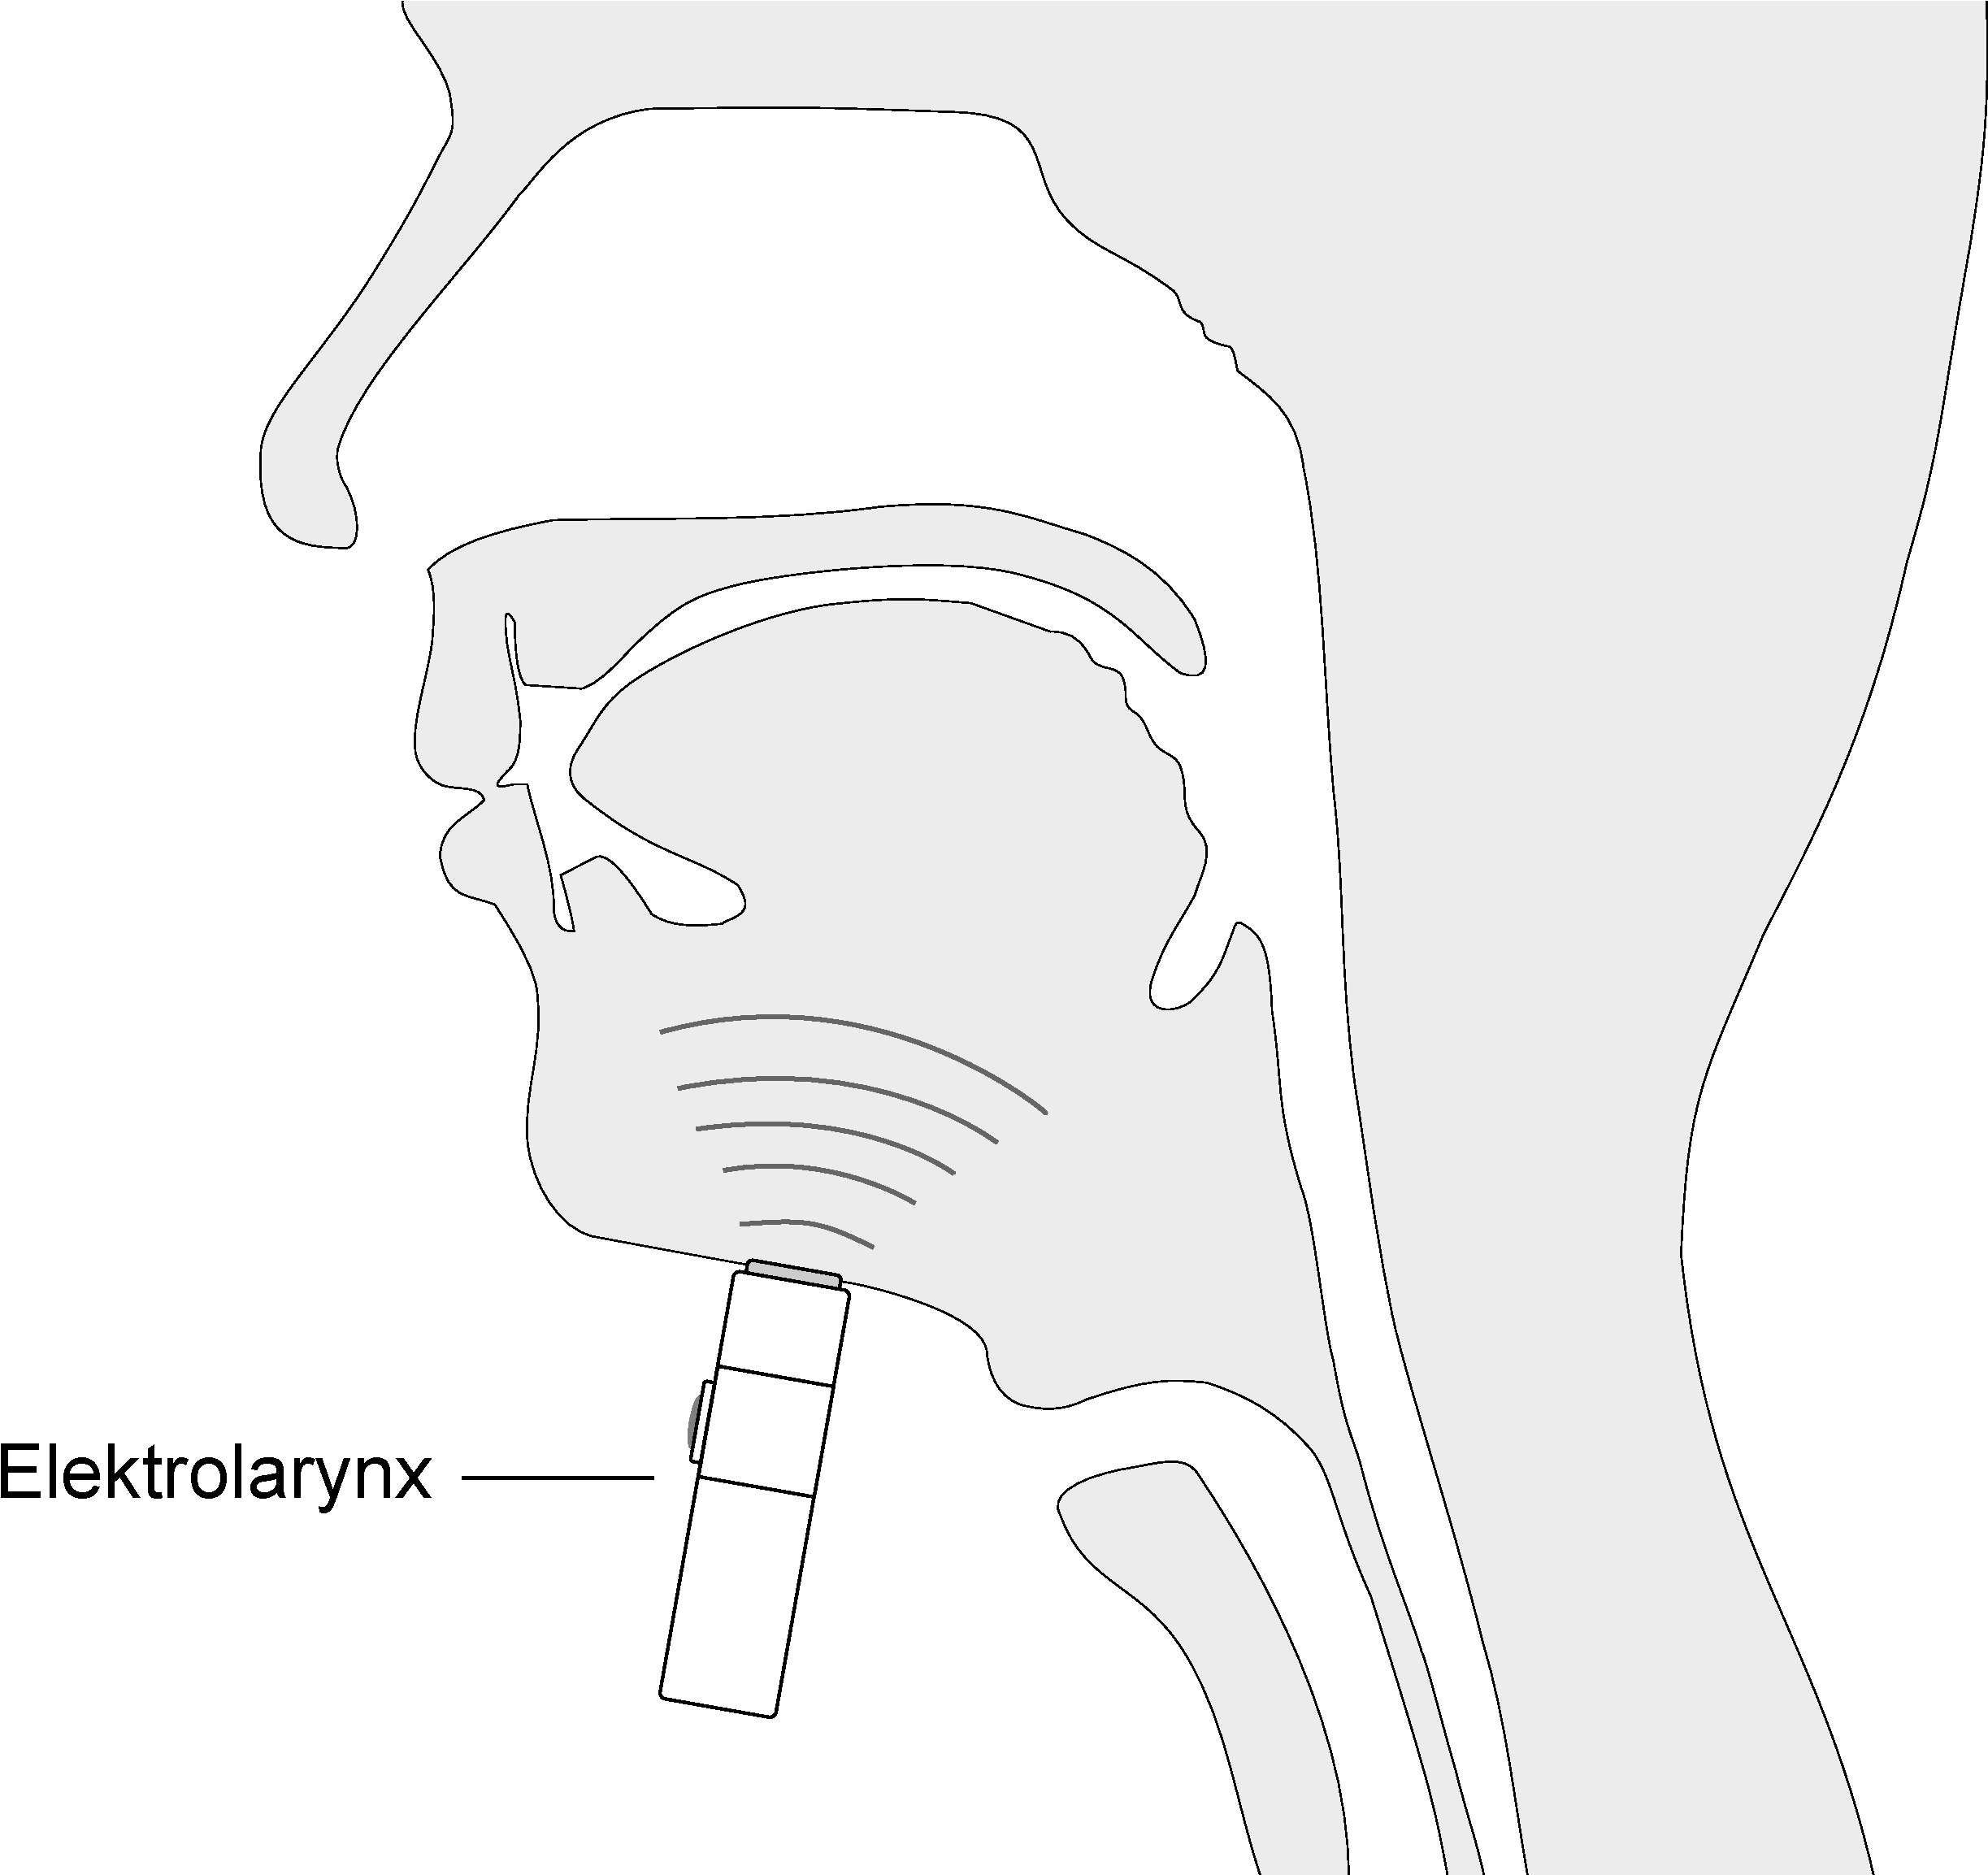
\includegraphics[width=0.6\linewidth]{ch3-cause/figures/electrolarynx}
    \caption[Princip rehabilitace hlasu pomocí elektrolarynxu.]{Princip rehabilitace hlasu pomocí elektrolarynxu.}
    \label{fig:cause:treatment:electrolarynx}
  \end{center}
\end{figure}

% TODO: ELEKTROLARYNX pasaze o monotonosti reci poradne promyslet

Takto generovaná řeč se vyznačuje několika charakteristickými rysy. V~první
řadě řeč budí velmi mechanický dojem. Důvodem je samozřejmě samotný
elektrolarynx, který lze označit za elektromechanický generátor zvuku s
konstantním buzením. Proto je také základní frekvence produkovaného hlasu víceméně konstantní a řečník tak má velmi omezené možnosti jak řeč emotivně zabarvovat. V~průběhu času se sice objevily snahy o ovlinění základní frekvence produkované řeči \cite{Kikuchi2004, Uemi1994, Goldstein2004}, kterou by bylo možné vyvolat prostřednictvím změny budící frekvence elektrolarynxu, ale ty ztroskotaly, jelikož jako velmi obtížné se jeví nalezení vhodného mechanismu, pomocí kterého by bylo docíleno optimální změny fundamentální frekvence mluvené řeči s~ohledem na to, co chce řečník říci. Dalším charakteristickým rysem hlasu produkovaného pomocí elektrolarynxu je jeho nižší srozumitelnost. K tomuto jevu dochází v~důsledku přítomnosti zvukového podkresu generovaného přístrojem. Srozumitelnost se navíc snižuje s~rostoucím okolním hlukem, proto se velmi často stává, že posluchač, který se s~takto produkovanou řečí setkává poprvé, není schopen promluvám plně porozumět.

Naproti tomu, za výhody, kterými tato metoda rehabilitace hlasu disponuje, lze označit možnost rychlého
osvojení schopnosti opětovně produkovat řeč. Navíc je vhodná pro téměř všechny pacienty
postižené ztrátou hlasu v~důsledku odstranění hrtanu popř. jeho poškození.
Za nevýhodu lze obecně pokládat kvalitu produkované řeči, tedy monotonní a
mechanicky znějící hlas. Za jistý způsob omezení lze považovat nutnost držení elektrolarynxu, jakožto přídavného zařízení, při mluvení.

% Samostatnou kapitolou může být psychologický dopad na pacienta. Stejně jako
% u~jícnového hlasu se řeč produkovaná promocí elektrolarynxu jeví odlišně od
%řeči přirozené. Navíc se ještě přidává potřeba využití nějakého zařízení.
% Člověk proto v~mnoha případech cítí ostych a bojí se na veřejnosti mluvit.

% subsubsection elektrolarynx (end)

% subsection subsection_name (end)

\subsection{Chirurgicko-protetická metoda} % (fold)
\label{chap:cause:treatment:tracheo}

Další možností, kterou lze využít pro rehabilitaci hlasu, je po odstranění hrtanu chirurgicky vytvořit průchod
mezi průdušnicí a jícnem tak, aby u tracheostomovaného člověka mohl opětovně proudit vzduch z plic do úst.
Princip metody spočívá v~tom, že pacient při výdechu zneprůchodní operativně vytvořený otvor (stoma) v~oblasti krku. Vzduch tak projde skrz fistuli do oblasti jícnu, naráží do jeho stěn a dochází  k~jeho rozvibrování. Následně jsou tyto vibrace modulovány pomocí artikulačních orgánů a vzniká řeč.

Historicky první zmínka o vytvoření fistule\footnote{fistule (česky píštěl) je abnormální
otvor mezi dvěma dutými orgány, nebo mezi dutým orgánem a kůží.} mezi
průdušnicí a jícnem pochází z~roku 1932. V~tomto roce doktor Guttman poprvé
vytvořil tracheoezofageání shunt\footnote{shunt - kanál, kterým je tekutina
odkloněna z přirozené dráhy. Tento kanál může být vytvořen chirurgicky nebo pomocí syntetické trubice. }.
Hlavní snahou chirurgů bylo vytvoření bezpečné, správně nasměrované píštěle
umožňující tvorbu hlasu. Bohužel v~mnoha případech byly zákroky doprovázené
vážnými komplikacemi (infekcemi, zápaly či těžkým krvácením).
Mimo to se museli operatéři vypořádat se zajištěním stálosti
vytvořeného otvoru tak, aby jím neprotékaly tekutiny špatným směrem a
nedocházelo  k~jejich zatékání do dýchacích cest. Jelikož se jednalo o velmi
náročné operační postupy a bylo s~nimi spojeno velké množství rizik, došlo v
80.~letech 20.~století  k~jejich ústupu. Svou renesanci zažily s~návrhem první protézy v~podobě jednocestného ventilu, který zajišťoval pouze jednosměrný
průchod tekutin skrze píštěl, jak je ilustrováno na obr.
\ref{fig:cause:treatment:shunt}. První komerčně dostupná protéza se objevila
v~80.~letech 20.~století v~USA.

\begin{figure}[htb]
  \begin{center}
    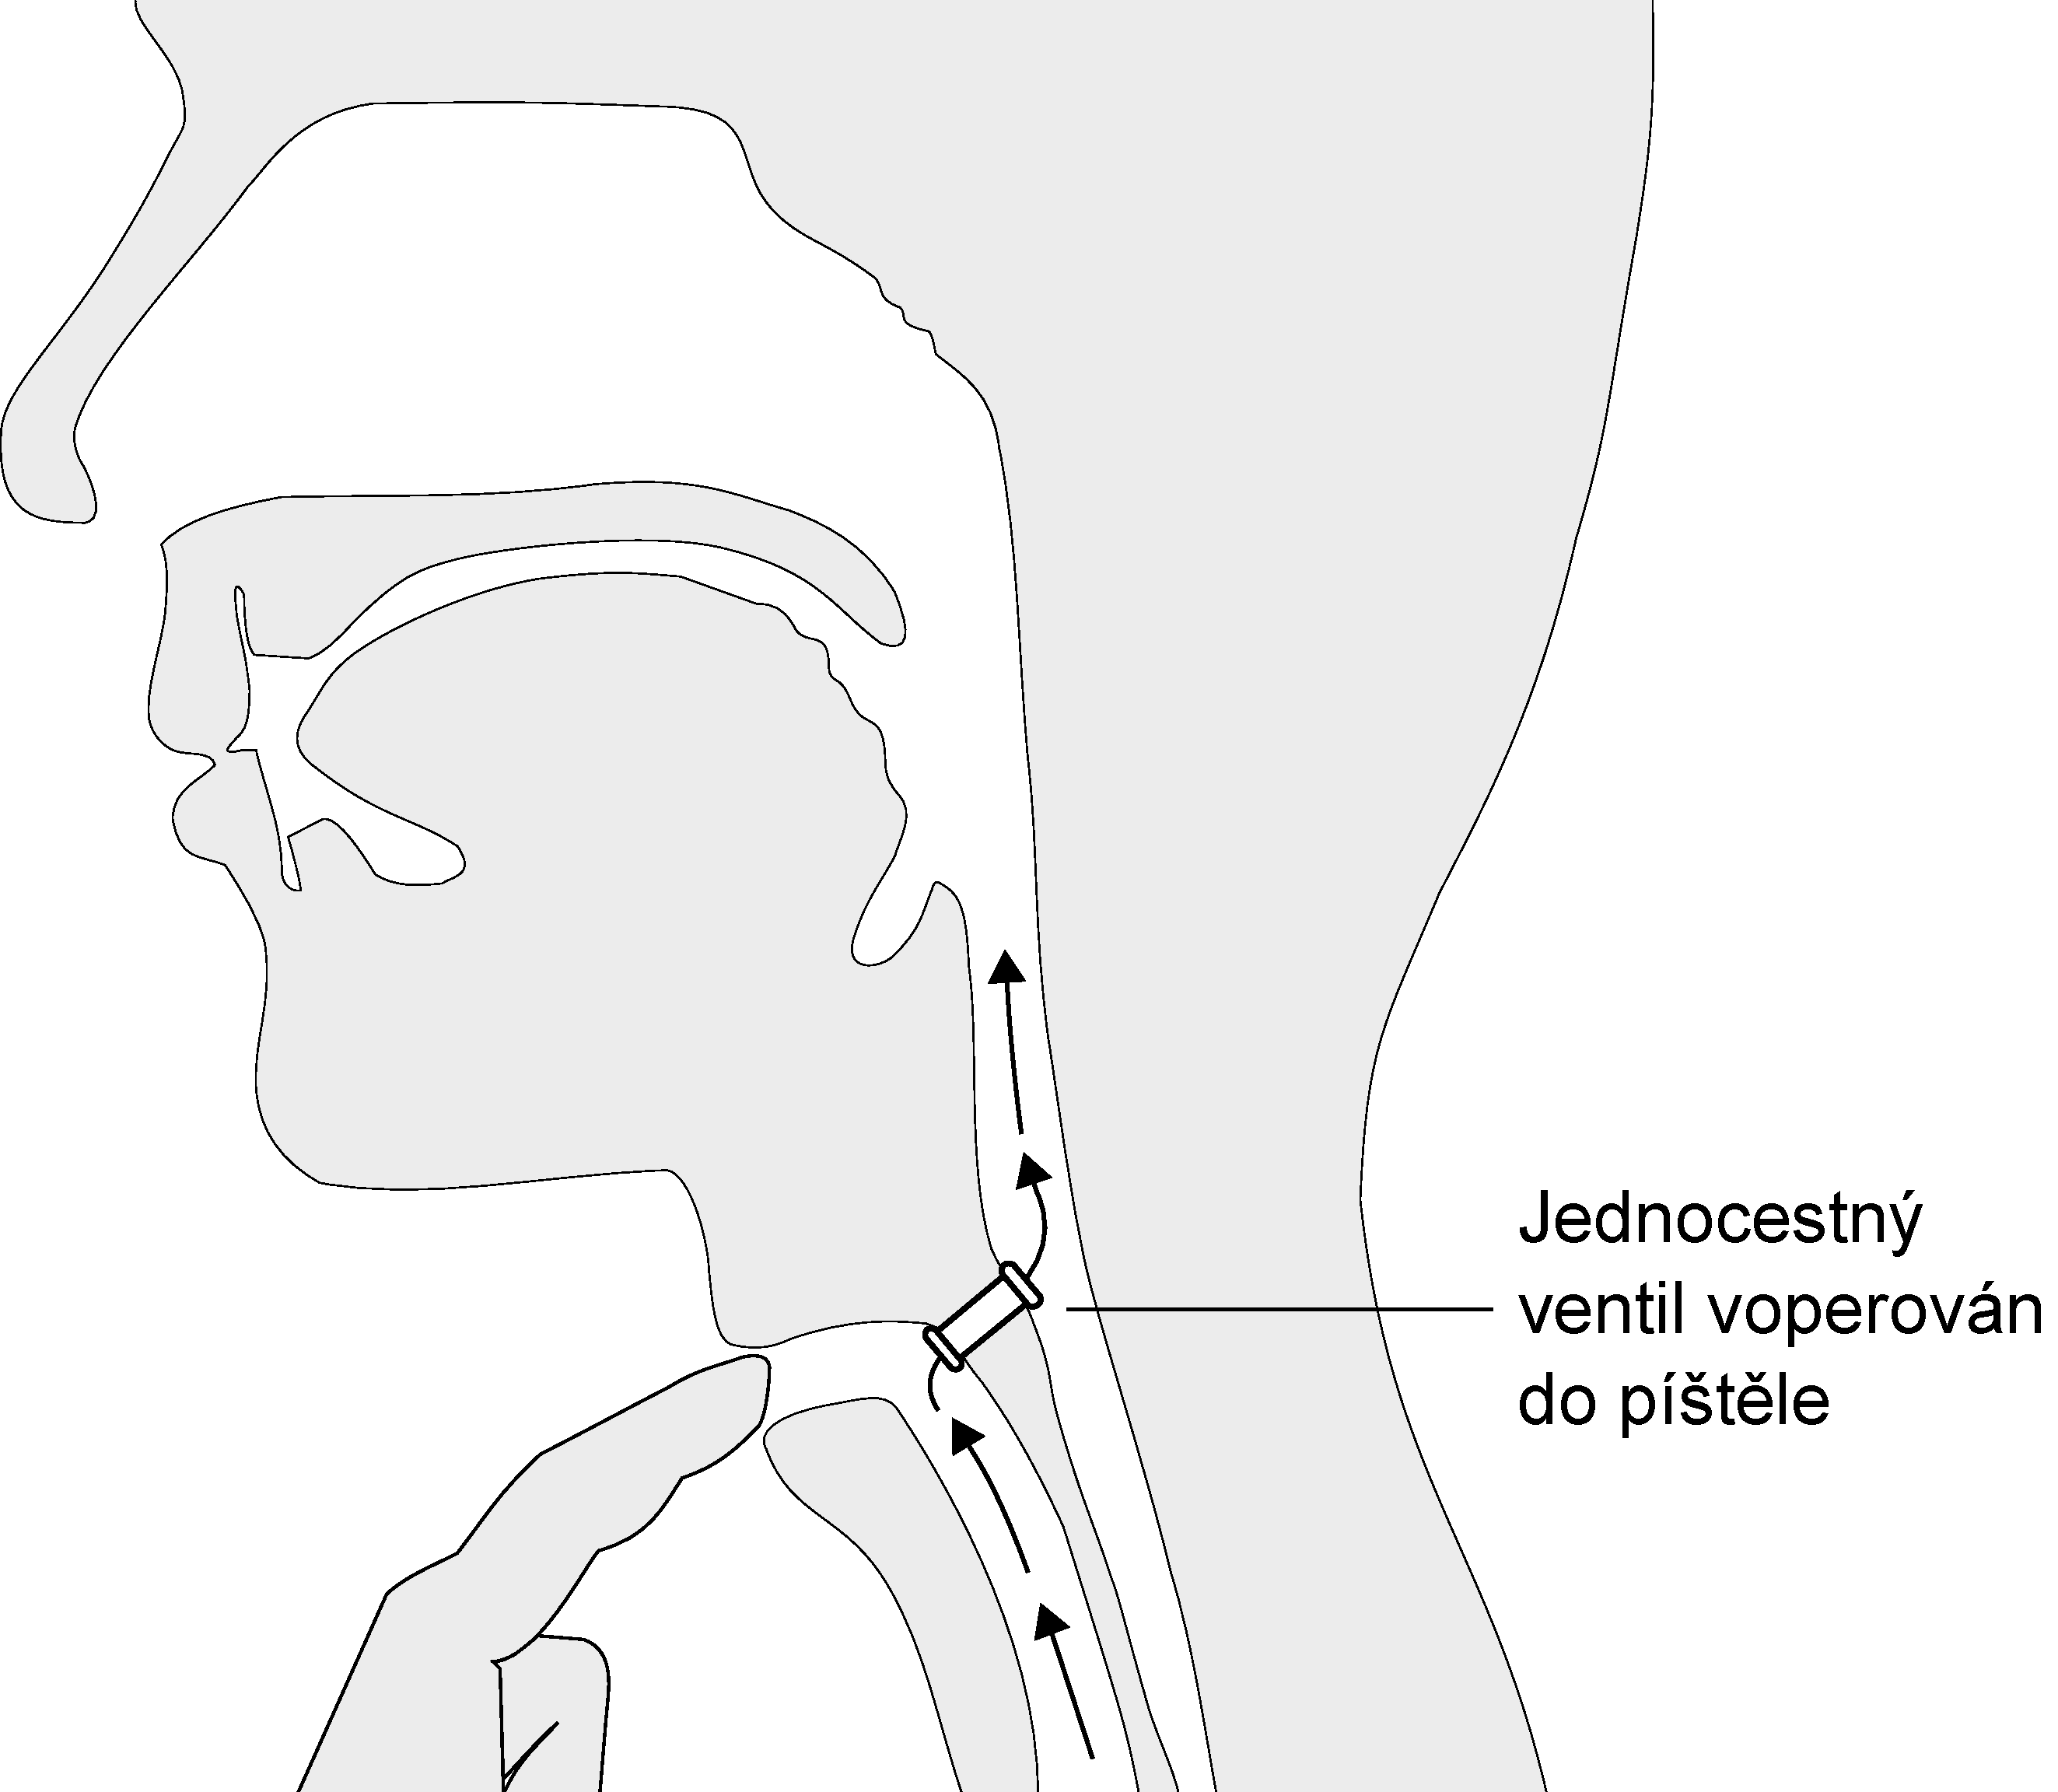
\includegraphics[width=0.6\linewidth]{ch3-cause/figures/te-shunt}
    \caption[Průchod vzduchu tracheoezofageální protézou.]{Průchod vzduchu tracheoezofageální protézou.}
    \label{fig:cause:treatment:shunt}
  \end{center}
\end{figure}


Na používané protézy jsou kladené
přísné nároky a musí vyhovovat určitým požadavkům. Musí být vyrobeny
z~biokompatibilního materiálu, který odolává biodegradaci. Tím je zaručena jejich
dlouhodobá trvanlivost a správná funkce. V~neposlední řadě by měla být protéza
samofixační a snadno vyměnitelná.
 K zajistění jejich správné funkce je zapotřebí navrhnout je tak, aby
tlak potřebný  k~otevření faryngoezofageálního segmentu byl co nejnižší. To by mělo zajišťovat pacientovi vytvářet
plynulou řeč. První vyráběné protézy se ale vyznačovaly tím, že tlak potřebný pro jejich otevření byl příliš vysoký a omezovaly tak množinu potencionálních pacientů. Nejmodernější protézy se již vyznačují
velmi nízkým otevíracím fonačním tlakem.

V praxi se používá několik druhů protéz. Hlavním rozdílem mezi nimi však je,
zda se pacient přímo účastní výměny ventilu, jehož fundamentální funkcí je
vytvoření průchodu pro vzduch proudící z průdušnice do jícnu. U protéz, které
jsou vyměňovány operačně, se doba používání pohybuje od 3 do 6 měsíců. Tento
interval velmi významně ovlivňuje tvorba biofilmu na povrchu náhrady. K tvorbě
dochází následkem přímého kontaktu protézy s~tělními tekutinami a potravou.
Rychlost tvorby biofilmu ovlivňuje tvar a materiál, ze kterého je náhrada
vytvořena \cite{Leunisse2001}. U typů, které si nositel může měnit sám, se
předpokládá, že budou čištěny nebo měněny přibližně jednou za dva týdny. Na obr. \ref{fig:cause:treatment:prosthesis} jsou
ukázány některé typy užívaných protéz.

\begin{figure}[htb]
  \begin{center}
    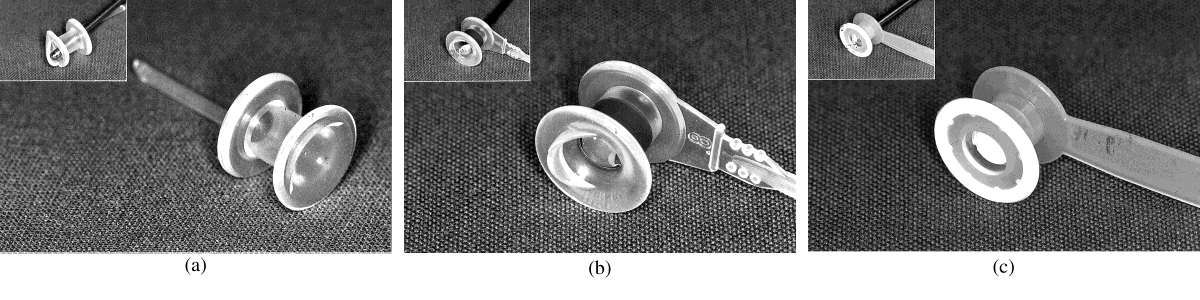
\includegraphics[width=0.9\linewidth]{ch3-cause/figures/te-protezy}
    \caption[Ilustrace používaných TE protéz.]{Ilustrace používaných TE protéz (a) Gronigenova nízkotlaká protéza, (b) Provox2 a (c) Blom-Singer protéza.}
    \label{fig:cause:treatment:prosthesis}
  \end{center}
\end{figure}


Samotný zákrok zavedení protézy je možné provést současně s~výkonem totální
laryngektomie (tzv. primární zavedení hlasové protézy) nebo až po zotavení
pacienta z~náročné léčby nádorového onemocnění (tzv. sekundární zavedení).
Primární zavedení umožňuje začít s~hlasovou rehabilitací krátce po odstranění
hrtanu. Zároveň pacient nemusí v~krátké době podstupovat druhou operaci, při
které by se vkládal jednocestný ventil do vytvořené fistule.



V praxi se ukázalo, že úspěšnost rehabilitace pomocí této metody je více než 80~\%
\cite{Slavicek2002}. Důležitým faktorem, stejně jako u metody jícnového hlasu, je
funkčnost faryngoezofageálního segmentu. Významnou roli hraje také otvírací tlak horního
jícnového svěrače. Hlas tvořený protézou se vyznačuje vysokou kvalitou, dobrou
srozumitelností, individuálním zabarvením a relativně dlouhou fonační dobou
dosahující průměrně 20 sekund \cite{Saito2003}. Oproti jícnovému hlasu není potřeba
tak intenzivní edukace pacienta k~plnému osvojení hlasu. V~současnosti se
jedná o nejpoužívanější metodu rehabilitace hlasu.

% TODO: Vyhody nevyhody metody - film tvorici se na proteze
% TODO: Kriteria na pacienta
% subsection chirurgicko_protetická_metoda (end)

\subsection{Hrtanu podobné struktury} % (fold)
\label{chap:cause:tratment:structure}

S rozvojem mikrovaskulárních\footnote{mikrovaskulární - část oběhového systému
složeného z nejmenších cév, jako jsou kapiláry, žilky aj.} transplantátů se
začaly objevovat postupy, které umožňovaly rehabilitovat hlas pouze pomocí
chirurgického zákroku. Tyto techniky jsou založeny na myšlence permanentního spojení hypofaryngu
s tracheou pomocí vlastní tkáně pacienta.

První metodu tohoto druhu představil v~roce 1984 doktor Ehrenberger
\cite{Kramp2009}, který popsal tzv. \uv{\textbf{řečový sifón}}
(angl. \textbf{speech siphon}). Jedná se o dvakrát esovitě zahnuté spojení mezi hrtanem a hltanem
vytvořené z části tenkého střeva zvané lačník (jejunum). Dvojesovité zahnutí je provedeno tak, aby
bylo minimalizováno riziko sekundární aspirace. Schéma \uv{řečového sifónu}
podle Ehrenberga je znázorněno na obr. \ref{fig:cause:treatment:microvascular}
A. Již na první pohled je zřejmé, že se jedná o velmi náročný chirurgický
zákrok. První články publikované autorským kolektivem prezentovaly velmi dobré
funkční výsledky metody. Podle \cite {Sebova-Sedenkova2006} bylo touto metodou doposud
operováno přibližně 60 pacientů.

V roce 1990 byla popsána laryngoplastika podle Hagena. V~tomto případě je za účelem vytvoření ústrojí zvaného \textbf{neolarynx} používán štěp z předloktí. Neoglottis je vyztužen chrupavkou
a překrývá vchod do neolaryngu tak, aby nedocházelo  k~sekundární aspiraci. Vnitřek neolaryngu je kryt kůží.
Laryngoplastika podle Hagena je znázorněna na obr.
\ref{fig:cause:treatment:microvascular} B. Doposud bylo touto metodou operováno přibližně 300
pacientů \cite{Sebova-Sedenkova2006}.

\begin{figure}[htb]
  \begin{center}
    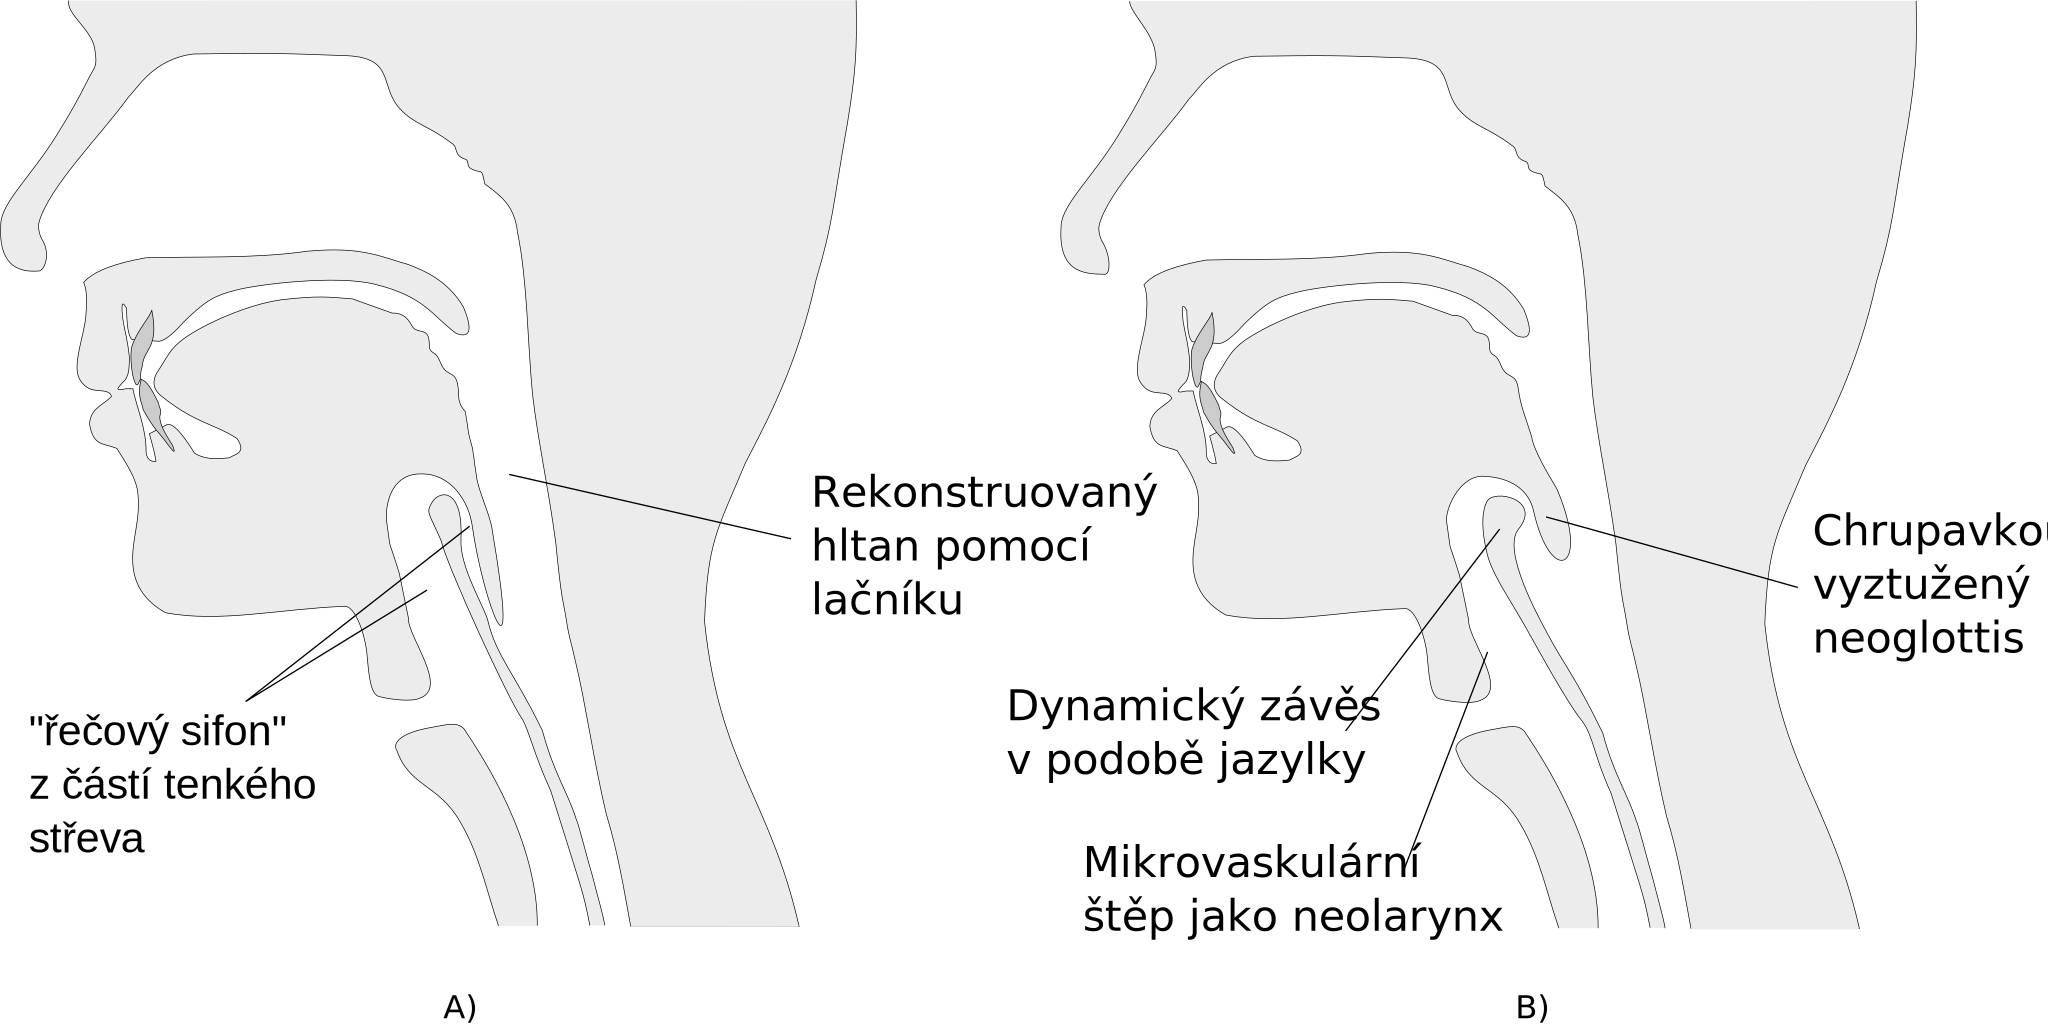
\includegraphics[width=0.9\linewidth]{ch3-cause/figures/microvascular}
    \caption[Schéma \uv{řečového sifónu} a laryngoplastiky.]{A) Schéma \uv{řečového sifónu} tak jak jej představil Ehrenberg. B) Laryngoplastika podle Hagena.}
    \label{fig:cause:treatment:microvascular}
  \end{center}
\end{figure}

Bohužel v~současné době tyto metody nenacházejí širší uplatnění. Hlavním důvodem je
náročnost realizace operačních postupů, kvůli které se velmi
těžko prosazují na dalších pracovištích. Dalším aspektem, který limituje tyto
metody, je vliv na samotného pacienta. Metody předpokládají provedení dalšího chirurgického
zákroku, který představuje pro pacienta další zátěž a mohou ho provázet nemalé komplikace.
I přes nedostatky těchto metod je
pochopitelná snaha lékařů o intenzivní výzkum v~této oblasti. Při úspěšné
léčbě je pacient schopen produkovat hlas velmi dobré kvality a ve většině
případů nepotřebuje žádnou péči ze strany lékařů.

% subsection hrtanu_podobné_struktury (end)

\subsection{Transplantace hrtanu}
\label{chap:cause:treatment:transplantation}

Nejkomplexnější možnost rehabilitace hlasu představuje transplantace hrtanu.
Pokud je úspěšná, přebírá transplantovaný orgán plně funkci původního
orgánu a velmi významně zvyšuje šance pacienta na plné zotavení bez trvalých
následků. Jedná se ale o velmi náročný chirurgický zákrok, protože je potřeba provést reinervaci a obnovení cévního zásobení implantátu.

Přestože první zmínky o možnosti provedení transplantace hrtanu se objevují již v~60.~letech 20.~století\footnote{Vůbec první úspěšná transplantace
orgánu (ledvin) se uskutečnila v~roce 1954.}, byla první transplantace tohoto druhu provedená
až profesorem Marshallem Stromem v~roce 1998 \cite{Narula2011},
Prvním pacientem, který podstoupil zmiňovaný chirurgický zákrok, byl čtyřicetiletý muž z USA.
K~laryngektomii v~jeho případě vedla motocyklová nehoda, při které došlo  k~rozdrcení hrtanu. Před transplantací pacient využíval 20 let  k~produkci řeči elektrolarynx. Dárcem orgánu byl taktéž čtyřicetiletý muž, který zemřel na následky prasknutí mozkového aneurysmatu. Příjemce transplantátu již třetí den po operaci promluvil (vyslovil
anglické slovo \uv{hello}). Přibližně po 36 měsících od transplantace byl
produkovaný hlas kvalitativně srovnatelný s~hlasem zdravého člověka. U této transplantace se však nepodařilo dosáhnout kompletní reinervace, proto nebylo možné zajistit bezproblémové dýchání a bylo proto nutné
ponechat tracheostomii. I přes tuto skutečnost měl zákrok významný podíl na zvýšení kvality jeho života
\cite{Strome2001}. Doposud poslední úspěšně vykonaná transplantace hrtanu byla
dle dostupných zdrojů provedena v~říjnu 2010.

%První informace spojené s~výzkumem možností provedení transplantace hrtanu se
%objevují již v~60. letech 20. století\footnote{Vůbec první úspěšná transplantace
%orgánu (ledvin) se uskutečnila v~roce 1954.}. Přesto byla první totální
%do dnešních dnů byly provedeny pouze 2 kompletní
%transplantace.

%Prvním pacientem, který podstoupil transplantaci, byl čtyřicetiletý muž z USA.
%K~laryngektomii v~jeho případě vedla motocyklová nehoda, při které si pacient
%rozdrtil hrtan. K incidentu došlo 20 let před transplantací. Před zákrokem
%používal k~produkci řeči elektrolarynx. Dárcem orgánu byl taktéž čtyřicetiletý
%muž, který zemřel na mozkové aneurysma. Úspěch transplantace se na příjemci
%projevil již třetí den po operaci, kdy poprvé po 20 letech promluvil (vyslovil
%anglické slovo \uv{hello}). Přibližně po 36 měsících od transplantace byl
%produkovaný hlas srovnatelný s~hlasem zdravého člověka. Podle vlastních slov
%pacienta se po operaci jeho kvalita života \uv{nesmírně} zlepšila.
%\cite{Strome2001} Doposud poslední úspěšně vykonaná transplantace byla
%zaznamenána v~říjnu 2010.

Jedním z hlavních důvodů tak nízkého počtu úspěšně provedených zákroků je, že se jedná o transplantaci dárcovského orgánu. Pacientům jsou podávány medikamenty zabraňující odmítnutí dárcovského orgánu (imunosupresiva), která ale v~současné době nelze podávat pacientům trpícím rakovinným onemocněním, protože významně zvyšují riziko opětovného rozšíření rakoviny \cite{Narula2011}. Ve výjimečných případech lze tuto metodu zvažovat u pacientů, kteří trpěli benigními nádory a minimálně 5~let u nich nedošlo  k~recidivě.
Poslední výzkumy však naznačují, že by v~dohledné době v~této oblasti mohlo dojít  k~pokroku, v~důsledku kterého by bylo možno provést transplantaci hrtanu i u lidí, kteří trpěli rakovinným onemocněním.

%Mezi hlavní důvody takto malého počtu zákroků patří množství pacientů vhodných
%pro tuto proceduru. Jelikož se jedná o transplantaci dárcovského orgánu je
%nutné použití imunosupresiv, tedy medikamentů zabraňující odmítnutí orgánu.
%Imunosupresiva jsou však v~současné době nepoužitelná u lidí trpících
%rakovinou hrtanu z důvodu velmi vysokého rizika rozšíření rakoviny
%\cite{Narula2011}.
%
%Poslední výzkum v~oblasti imunosuprese však naznačuje, že by v~dohledné době
%mohlo dojít  k~pokroku a umožnit transplantaci hrtanu i u lidí trpících
%rozsáhlou rakovinou v~oblasti krku \cite{Narula2011}. Prozatím je však tato
%metoda vhodná pro pacienty netrpící rakovinou, případně ty, u kterých
%převažovaly benigní nádory a již 5 let nedošlo  k~recidivě.

% subsection transplantace_hrtanu (end)

\subsection{Shrnutí} % (fold) \label{sub:treatment:summary}

% NOTE: Neni lepsi pouzit dusledky misto nasledky 3

Rehabilitaci hlasu u pacientů, kteří prodělali chirurgické odstranění hrtanu, je ve
vyspělých zemích věnována značná pozornost, jelikož následky této operace velmi významně ovlivňují kvalitu jejich života. Léčení jedinci se musí vyrovnat primárně se ztrátou hlasu. V~některých případech dochází po operaci i ke ztrátě čichu a pacienti jsou náchylnější ke vzniku respiračních onemocnění.
Tato situace je již sama o sobě velmi náročnou psychickou zkouškou. Neméně významnou
roli sehrává i fyzická odlišnost a z~toho pramenící psychická zátěž, které je pacient vystaven
po absolvované léčbě.

 V~současnosti je za účelem rehabilitace hlasu využíváno několik metod, jejichž přehled je spolu s~jejich hlavními výhodami a nevýhodami uveden v~tabulce v~tab. \ref{tab:treatment:summary}.
%Nejpoužívanějšími z nich jsou \textbf{tracheoezofageální
%píštěl} (popsáno v~části \ref{chap:cause:treatment:tracheo}), \textbf{jícnový
%hlas} (\ref{chap:cause:treatment:foniatric:esophageal}) a použití
%\textbf{elektrolarynxu} (\ref{chap:cause:treatment:foniatric:elektrolarynx}).
U většiny pacientů je hlas rehabilitován pomocí metody tracheoezofageálního píštěle,
která je principiálně založena na metodě jícnového hlasu. O úspěchu rehabilitace, stejně jako u jícnového hlasu, tak
především rozhodují vlastnosti faryngoezofageálního segmentu. Pokud si pacient
není schopen osvojit techniku jícnového hlasu, případně nemá voperován píštěl, je
pro rehabilitaci hlasu použit elektrolarynx. Za nejkomplexnější ze zmíněných postupů se dá považovat úplná transplantace hrtanu, která
řeší víceméně všechny problémy spojené s~odstraněním hrtanu. Bohužel tento
zákrok je velmi náročný a vhodný pouze pro omezený okruh pacientů.

\newcolumntype{b}{X}
\newcolumntype{s}{>{\hsize=.5\hsize}X}

\begin{table}[ht]
  \centering
  \begin{tabularx}{1.0\textwidth}{L{1.2} L{0.6} L{1.1} L{1.1}}
    & \textbf{Kvalita} & \textbf{Výhody} & \textbf{Nevýhody} \\
    \toprule \\ [-1.75ex]

    \textbf{Tracheoezofageální píštěl} & Vysoká & Vysoká míra osvojení, dlouhá fonační doba & Zanášení píštěle a s~ním spojené čištění, případně dodatečná lékařská péče \\
    \midrule \\ [-1.75ex]

    \textbf{Jícnový hlas} & Dobrá & Volné ruce při mluvení, není potřeba dodatečné lékařské péče & Velmi náročná metoda  k~naučení, nepřirozený hlas \\
    \midrule \\ [-1.75ex]

    \textbf{Elektrolarynx} & Nízká & Snadné  k~naučení & Monotonní až robotický hlas, nutné nosit externí elektrické zařízení \\
    \midrule \\ [-1.75ex]

    \textbf{Hrtanu podobné struktury} & Vysoká & Nezávislost pacienta na pravidelné lékařské péči & Velmi náročná chirurgická procedura, která pacienta vystavuje dalším možným rizikům  \\
    \midrule \\ [-1.75ex]

    \textbf{Transplantace hrtanu} & Velmi vysoká & Transplantovaný hrtan přejímá funkci odstraněného orgánu & Velmi náročná chirurgická procedura, která je vhodná jen pro malé procento pacientů \\
  \end{tabularx}

  \caption{Přehled dostupných metod rehabilitace hlasu. \label{tab:treatment:summary}}
\end{table}

%Bohužel všechny výše zmíněné metody neřeší další problémy spojené s
%odstraněním hrtanu, a proto se lékaři stále snaží  rehabilitační metody zdokonalovat.
Přestože lékařská věda v~současnosti disponuje možnostmi jak rehabilitovat hlas a lékaři se snaží využívané postupy neustále zdokonalovat, zůstává zde otevřený prostor pro inovace, a tím zlepšení kvality života lidí postižených ztrátou hrtanu.
%
%
%
%Většina pacientů je tedy rehabilitována pomocí tracheoezofageálního píštěle,
%který principiálně vychází z jícnového hlasu, jehož negativa se snaží
%eliminovat. O úspěchu rehabilitace, stejně jako u jícnového hlasu, tak
%především rozhodují vlastnosti faryngoezofageálního segmentu. Pokud pacient
%není schopen si osvojit jícnový hlas, případně nemá voperován píštěl, je
%použit elektrolarynx. Bohužel tyto metody neřeší další problémy spojené s
%odstraněním hrtanu, a proto se lékaři stále snaží zdokonalovat rehabilitační
%metody. Za nejkomplexnější se dá považovat úplná transplantace hrtanu, která
%řeší víceméně všechny problémy spojené s~odstraněním hrtanu. Bohužel tento
%zákrok je velmi náročný a vhodný pouze pro malou část pacientů.
%I když je tedy v~současné době lékařská věda schopna rehabilitovat hlas, tak
%zde zůstává otevřený prostor pro inovace, a tím zlepšení kvality života lidí
%postižených ztrátou hrtanu.

% subsection treatment:summary (end)

% section rehabilitace_hlasu_po_totalni_laryngektomii (end)
